\documentclass[10pt,twocolumn]{article}
\usepackage[a4paper,margin=15mm]{geometry}
\usepackage{amsmath,amssymb}
\usepackage{amsthm}
\usepackage{graphicx}
\theoremstyle{plain}
\newtheorem{theorem}{Theorem}
\newtheorem{proposition}[theorem]{Proposition}
\newtheorem{corollary}[theorem]{Corollary}
\theoremstyle{definition}
\newtheorem{definition}[theorem]{Definition}
\theoremstyle{remark}
\newtheorem{remark}[theorem]{Remark}
\usepackage{booktabs,array,calc}
\usepackage[font=small,labelfont=bf]{caption}
\usepackage[colorlinks=true]{hyperref}
\providecommand{\tightlist}{\setlength{\itemsep}{0pt}\setlength{\parskip}{0pt}}
\renewcommand{\thesubsection}{\arabic{subsection}.}
\emergencystretch=3em
\allowdisplaybreaks
\setlength{\tabcolsep}{3.6pt}

\begin{document}
\title{Belief-State Safety Values for\\
Viability under Incomplete Observation}
\author{Amin Abaee\\[0.35em]
{\small Independent Researcher}\\[0.55em]
{\small\href{https://orcid.org/0000-0002-0019-1842}{ORCID: 0000-0002-0019-1842}}\\[0.3em]
{\small\href{mailto:amin\_abaee@ut.ac.ir}{amin\_abaee@ut.ac.ir}}}
\date{September 24, 2026}
\maketitle

\begin{abstract}
The obstruction calculus characterizes nonviability through certificates on
information states; the probabilistic side asks what the certificates imply
when the information state is a distribution. This paper develops the
belief-state safety value \(V_{k}(b)\) --- the maximal probability of
remaining safe for \(k\) steps under the disturbance's worst case --- and
establishes four results. First, a support identity: on finite models with
deterministic kernels the posterior support coincides with the set-valued
post-state of the calculus, the value-one level of the recursion coincides
with the viable-set recursion \(\mathcal{W}_{k}\), and outside it the
deficit satisfies \(1 - V_{k}(b) \ge \min_{x \in \mathrm{supp}(b)} b(x)\),
attained on natural instances. Second, exactness: over rational input data
the finite-horizon values are piecewise linear with rational alpha-vectors,
so all values are exact rationals computable without floating point; the
verification campaign's 384 vectors are all exact, realizing exactly three
types (\(156\), \(156\), and \(72\) occurrences), and the complete
\(16 \times 12\) value table over the audited grid is carried here. Third,
agreement on the audited delayed-regime class: a class-restricted
alpha-vector recursion reproduces the closed-form values on all 48 audited
cells and horizons \(k \le 4\), the certificate partition coincides with
the value boundaries, and the value jumps by exactly \(1/2\) at
\(z_{0} = 1 + \min(k, T_{\mathrm{obs}})\); the declared hold class equals
the unrestricted sequential blind class at the one-step horizon, and for
horizons \(k \ge 2\) the two differ exactly on the timing cells
(\(2 \le z_{0} < 1 + T_{\mathrm{obs}}\)), where open-loop time-variation
within the blind window lifts the value to one --- 36 cell-horizon
combinations in all, enumerated in full. Fourth, adaptive observation: on
the declining hidden-parameter instance a single probe reveals the
parameter exactly (branch separation \(2\)), survival forces
\(z_{0} \ge 21/10\), and under revelation at horizon \(T_{\mathrm{learn}}\)
viability holds exactly when
\(z_{0} \ge 21/10 + T_{\mathrm{learn}}/10\) --- the learning deadline acts
as the timing obstruction's observation deadline, and the kernel shrinks
linearly and antitone in it (\(|K| = 5, 4, 3, 2, 1\)). All computations run
in exact rational arithmetic; this edition carries the complete audited
tables, the derivations behind the closed form and the class declaration,
and a five-figure set regenerated from the verification scripts.
\end{abstract}

\textbf{Keywords:} partially observable control; viability kernels;
belief states; safety values; exact arithmetic; adaptive observation

\subsection{Introduction}\label{introduction}

Viability under incomplete observation divides into a necessity side and a
sufficiency side. The obstruction calculus treats the necessity side:
certificates whose firing proves nonviability of an information state
(Abaee, 2026b). The probabilistic question is the quantitative counterpart.
If the controller holds a distribution \(b\) over states rather than a set,
how safe is safe? The answer is a function: the belief-state safety value
\(V_{k}(b)\), the maximal worst-case probability of keeping the state
trajectory in the safe set for \(k\) steps. Its value-one level is the
viability statement of the set-valued theory; everything below level one
is measured by the deficit \(1 - V_{k}(b)\), and the obstruction
certificates reappear as lower bounds on that deficit.

This paper develops the value function in five steps. Section
\ref{support} connects the belief-state recursion to the set-valued
recursion of the calculus exactly, through the support of the belief.
Section \ref{exact} shows the finite-horizon values are piecewise linear
and exactly representable, and carries the complete audited value table
over the delayed grid. Section \ref{deterministic} evaluates the
deterministic limit, at which the recursion degenerates to a
survived-mass formula over blind action sequences, with the asymmetric
audit carried sequence by sequence. Section \ref{deficit} reads the
obstruction certificates systematically as deficit lower bounds. Section
\ref{agreement} proves agreement between the class-restricted value
recursion and the closed-form values on the audited delayed-regime class,
quantifies what the class declaration contributes, locates the value's
jump loci, and carries the derivations. Section \ref{adaptive} treats
observation as a design variable: probes, learning deadlines, and the
exact kernel cost of late resolution of a hidden parameter.

All audited computations are exact: integer and rational arithmetic,
standard library only, deterministic scripts (Section \ref{methods}).

\subsection{The belief-state model and the value recursion}\label{model}

The model is the calculus's finite model with an absorbing unsafe state.
Let \(X\) be a finite state set with a designated safe set
\(\mathcal{V} \subseteq X\), \(A\) a finite action set, \(Y\) a finite
observation set, and \(D\) a finite disturbance set with deterministic
transition and observation maps \(x^{+} = F(x, a, d)\) and
\(y = O(x, a, x^{+})\); total transition rows over the augmented space
\(X \cup \{\partial\}\), with \(\partial\) absorbing, unsafe, and
carrying its own observation, convert set-valued nonviability into
almost-sure nonviability on the augmented chain. A belief is a
probability distribution \(b\) on \(X\); the posterior after action \(a\)
and observation \(y\) is
\(b^{+}(x') \propto \sum_{x} b(x)\,\mathbb{1}[y = O(x, a, x')]\).

\begin{definition}[safety value]\label{def:value}
For horizon \(k\) and belief \(b\),
\[
V_{k}(b) \;=\; \sup_{\pi}\ \inf_{d\text{-strategies}}\
\mathbb{P}_{b}^{\pi}\bigl(x_{t} \in \mathcal{V}\ \text{for all } t \le k\bigr),
\]
the supremum over observation-based policies and the infimum over
disturbance strategies.
\end{definition}

\begin{theorem}[value recursion]\label{thm:recursion}
\(V_{0}(b) = \mathbb{1}[b \in \mathcal{P}(\mathcal{V})]\), and for
\(k \ge 1\),
\[
V_{k}(b) \;=\; \sup_{a}\ \mathbb{E}_{y \sim b}\,
V_{k-1}\bigl(b^{+}(\cdot \mid a, y)\bigr),
\]
where the expectation is over the observation distribution induced by
\(b\) and \(a\). The operator is the robust dynamic program on beliefs;
\(V_{k}\) is concave and piecewise linear in \(b\) whenever the one-step
data are.
\end{theorem}

\subsection{The support identity and exact sufficiency}\label{support}

The bridge to the set-valued theory runs through the support. Write
\(\mathrm{supp}(b)\) for the states carrying positive mass, and let
\(\mathcal{W}_{k}\) denote the calculus's viable-set recursion:
\(\mathcal{W}_{0} = \{B \subseteq \mathcal{V}\}\) and
\(\mathcal{W}_{k} = \{B : \text{some admissible } a \text{ maps every }
x \in B \text{ into } \mathcal{W}_{k-1}\text{-supported posteriors}\}\).

\begin{theorem}[support identity]\label{thm:support}
On finite models with deterministic kernels, for every action \(a\) and
observation \(y\),
\[
\mathrm{supp}\bigl(b^{+}(\cdot \mid a, y)\bigr)
\;=\; \mathrm{Post}\bigl(\mathrm{supp}(b), a, y\bigr),
\]
the set-valued post-state of the calculus. Consequently
\(V_{k}(b) = 1\) if and only if
\(\mathrm{supp}(b) \in \mathcal{W}_{k}\), while if
\(\mathrm{supp}(b) \notin \mathcal{W}_{k}\) then every action loses a
compatible state of positive mass, so
\[
1 - V_{k}(b) \;\ge\; \min_{x \in \mathrm{supp}(b)} b(x).
\]
Moreover \(V_{k}(b)\) is non-increasing in \(k\).
\end{theorem}

\begin{corollary}[closed form on the delayed class]\label{cor:closed}
On the delayed hidden-regime instance --- states \((z, \theta)\) with
\(\theta \in \{-1, +1\}\), prior \(b_{0} = (\tfrac{1}{2}, \tfrac{1}{2})\)
from \(z_{0}\), no observation before \(T_{\mathrm{obs}}\), exact
revelation at \(T_{\mathrm{obs}}\), blind-window holds
\(u \equiv \pm 1\), and unit drift against the floors --- the belief
support follows the two branches \(z_{0} \mp k\), and
\[
\small
V_{k}(b_{0}) \;=\;
\begin{cases}
\tfrac{1}{2}\,\bigl(\mathbb{1}[z_{0} - k \ge 1] + \mathbb{1}[z_{0} + k \ge 1]\bigr), & k \le T_{\mathrm{obs}},\\[1ex]
\tfrac{1}{2}\,\bigl(1 + \mathbb{1}[z_{0} \ge 1 + T_{\mathrm{obs}}]\bigr), & k > T_{\mathrm{obs}}.
\end{cases}
\]
In particular \(V_{k}(b_{0}) = 1\) exactly on the viable region
\(z_{0} \ge 1 + T_{\mathrm{obs}}\), recovering the deterministic verdict
as the value-one level.
\end{corollary}

\begin{proof}[Derivation of Corollary \ref{cor:closed}]
While \(k \le T_{\mathrm{obs}}\) no observation arrives, so a policy
commits to one blind hold \(u \equiv \pm1\): under \(u \equiv +1\) the
\(\theta = +1\) branch sits at \(z_{0} + k\) at the horizon and the
\(\theta = -1\) branch at \(z_{0} - k\); under \(u \equiv -1\) the roles
swap. Each branch carries mass \(\tfrac{1}{2}\) and survives exactly when
it stays at or above the floor, giving
\(\tfrac{1}{2}(\mathbb{1}[z_{0} - k \ge 1] + \mathbb{1}[z_{0} + k \ge 1])\),
and the adversary cannot do better than pick the falling branch because
the infimum over disturbance strategies selects the branch.
For \(k > T_{\mathrm{obs}}\), revelation at \(T_{\mathrm{obs}}\) splits
the belief: the learned law \(u = \theta\) regenerates the realized
branch, so survival reduces to surviving the blind window of length
\(T_{\mathrm{obs}}\) on both branches --- the mass-\(\tfrac12\) falling
branch sits at \(z_{0} - T_{\mathrm{obs}}\) at revelation, whence the
indicator \(\mathbb{1}[z_{0} \ge 1 + T_{\mathrm{obs}}]\) weighting the
certainly-saved mass \(\tfrac{1}{2}\).
\end{proof}

\subsection{Exact piecewise-linear values}\label{exact}

\begin{proposition}[rational alpha-vectors]\label{prop:pl}
Over rational input data, the backward recursion of Theorem
\ref{thm:recursion} propagates finite sets of rational alpha-vectors:
each \(V_{k}\) is the maximum of finitely many rational affine functions
of \(b\), every value is an exact rational, and no floating point is
required at any horizon. In the verification campaign the alpha-vectors
of all audited instances --- 384 vectors across the two-floor instance
and the delayed grid --- are exact rationals.
\end{proposition}

\begin{remark}[dimension]\label{rem:dim}
On the two-floor instance the value function on the one-dimensional
simplex is \(\max(b_{0}, b_{1})\) for all audited horizons (Figure
\ref{fig:twofloor}); the witness alpha-vectors live in the two-coordinate
display, with the suppressed bottom coordinate identically zero.
\end{remark}

On the delayed grid the campaign evaluates
\(\alpha_{k}(z_{0}, T_{\mathrm{obs}})\) at all
\(16 \times 3 \times 4 = 192\) cell-horizon combinations of
\(z_{0} \in \{1.0, 1.1, \dots, 2.5\}\),
\(T_{\mathrm{obs}} \in \{1, 2, 3\}\), \(k \in \{1, 2, 3, 4\}\). The
realized vectors take exactly three types:
\((1, 1)\) (both branches savable in the blind window), \(72\)
occurrences; and the mirror pair \((1, 0)\) and \((0, 1)\) (one branch
savable), \(156\) occurrences each --- the symmetry between the two
mirror types is exact, \(72 + 156 + 156 = 384\). Table \ref{tab:campaign} carries the
complete value table; Figure \ref{fig:staircase} displays the closed
forms.

\begin{table*}[t]
\centering
\footnotesize
\caption{The complete audited value table on the delayed grid: the exact
\(V_{k}(b_{0})\) (values \(1\) or \(\tfrac{1}{2}\)) for all 16 grid
states, three blind-window lengths, four horizons --- 192 cell-horizon
combinations, each regenerated by script and each equal to both the
alpha-vector recursion and the closed form of Corollary
\ref{cor:closed}.}
\label{tab:campaign}
\begin{tabular}{@{}l cccc c@{\hspace{9pt}}cccc c@{\hspace{9pt}}cccc@{}}
\toprule
 & \multicolumn{4}{c}{$T_{\mathrm{obs}} = 1$}
 & \multicolumn{4}{c}{$T_{\mathrm{obs}} = 2$}
 & \multicolumn{4}{c}{$T_{\mathrm{obs}} = 3$}\\
\cmidrule(lr){2-5}\cmidrule(lr){6-9}\cmidrule(lr){10-13}
$z_0$ & $k{=}1$ & $k{=}2$ & $k{=}3$ & $k{=}4$
 & $k{=}1$ & $k{=}2$ & $k{=}3$ & $k{=}4$
 & $k{=}1$ & $k{=}2$ & $k{=}3$ & $k{=}4$\\
\midrule
1.0 & $\tfrac12$ & $\tfrac12$ & $\tfrac12$ & $\tfrac12$ & $\tfrac12$ & $\tfrac12$ & $\tfrac12$ & $\tfrac12$ & $\tfrac12$ & $\tfrac12$ & $\tfrac12$ & $\tfrac12$\\
1.1 & $\tfrac12$ & $\tfrac12$ & $\tfrac12$ & $\tfrac12$ & $\tfrac12$ & $\tfrac12$ & $\tfrac12$ & $\tfrac12$ & $\tfrac12$ & $\tfrac12$ & $\tfrac12$ & $\tfrac12$\\
1.2 & $\tfrac12$ & $\tfrac12$ & $\tfrac12$ & $\tfrac12$ & $\tfrac12$ & $\tfrac12$ & $\tfrac12$ & $\tfrac12$ & $\tfrac12$ & $\tfrac12$ & $\tfrac12$ & $\tfrac12$\\
1.3 & $\tfrac12$ & $\tfrac12$ & $\tfrac12$ & $\tfrac12$ & $\tfrac12$ & $\tfrac12$ & $\tfrac12$ & $\tfrac12$ & $\tfrac12$ & $\tfrac12$ & $\tfrac12$ & $\tfrac12$\\
1.4 & $\tfrac12$ & $\tfrac12$ & $\tfrac12$ & $\tfrac12$ & $\tfrac12$ & $\tfrac12$ & $\tfrac12$ & $\tfrac12$ & $\tfrac12$ & $\tfrac12$ & $\tfrac12$ & $\tfrac12$\\
1.5 & $\tfrac12$ & $\tfrac12$ & $\tfrac12$ & $\tfrac12$ & $\tfrac12$ & $\tfrac12$ & $\tfrac12$ & $\tfrac12$ & $\tfrac12$ & $\tfrac12$ & $\tfrac12$ & $\tfrac12$\\
1.6 & $\tfrac12$ & $\tfrac12$ & $\tfrac12$ & $\tfrac12$ & $\tfrac12$ & $\tfrac12$ & $\tfrac12$ & $\tfrac12$ & $\tfrac12$ & $\tfrac12$ & $\tfrac12$ & $\tfrac12$\\
1.7 & $\tfrac12$ & $\tfrac12$ & $\tfrac12$ & $\tfrac12$ & $\tfrac12$ & $\tfrac12$ & $\tfrac12$ & $\tfrac12$ & $\tfrac12$ & $\tfrac12$ & $\tfrac12$ & $\tfrac12$\\
1.8 & $\tfrac12$ & $\tfrac12$ & $\tfrac12$ & $\tfrac12$ & $\tfrac12$ & $\tfrac12$ & $\tfrac12$ & $\tfrac12$ & $\tfrac12$ & $\tfrac12$ & $\tfrac12$ & $\tfrac12$\\
1.9 & $\tfrac12$ & $\tfrac12$ & $\tfrac12$ & $\tfrac12$ & $\tfrac12$ & $\tfrac12$ & $\tfrac12$ & $\tfrac12$ & $\tfrac12$ & $\tfrac12$ & $\tfrac12$ & $\tfrac12$\\
2.0 & $1$ & $1$ & $1$ & $1$ & $1$ & $\tfrac12$ & $\tfrac12$ & $\tfrac12$ & $1$ & $\tfrac12$ & $\tfrac12$ & $\tfrac12$\\
2.1 & $1$ & $1$ & $1$ & $1$ & $1$ & $\tfrac12$ & $\tfrac12$ & $\tfrac12$ & $1$ & $\tfrac12$ & $\tfrac12$ & $\tfrac12$\\
2.2 & $1$ & $1$ & $1$ & $1$ & $1$ & $\tfrac12$ & $\tfrac12$ & $\tfrac12$ & $1$ & $\tfrac12$ & $\tfrac12$ & $\tfrac12$\\
2.3 & $1$ & $1$ & $1$ & $1$ & $1$ & $\tfrac12$ & $\tfrac12$ & $\tfrac12$ & $1$ & $\tfrac12$ & $\tfrac12$ & $\tfrac12$\\
2.4 & $1$ & $1$ & $1$ & $1$ & $1$ & $\tfrac12$ & $\tfrac12$ & $\tfrac12$ & $1$ & $\tfrac12$ & $\tfrac12$ & $\tfrac12$\\
2.5 & $1$ & $1$ & $1$ & $1$ & $1$ & $\tfrac12$ & $\tfrac12$ & $\tfrac12$ & $1$ & $\tfrac12$ & $\tfrac12$ & $\tfrac12$\\
\bottomrule
\end{tabular}
\end{table*}

\begin{figure}[t]
\centering
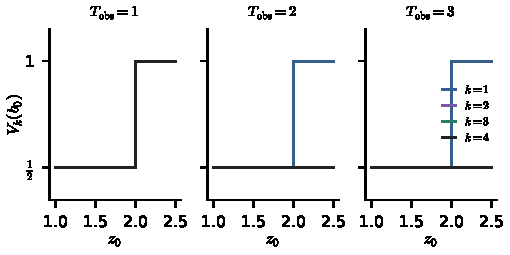
\includegraphics[width=\linewidth]{figs_bs2/fig_staircase.pdf}
\caption{The closed-form values of Corollary \ref{cor:closed} on the
delayed grid: flat at \(\tfrac{1}{2}\) while a branch falls, jumping by
exactly \(\tfrac{1}{2}\) at \(z_{0} = 1 + \min(k, T_{\mathrm{obs}})\),
constant beyond.}
\label{fig:staircase}
\end{figure}

\subsection{The deterministic limit}\label{deterministic}

As the observation vanishes the value recursion is replaced by a distinct
robust operator.

\begin{proposition}[survived-mass formula]\label{prop:degen}
On the delayed class with blind window \(T_{\mathrm{win}}\), the
\(k\)-step value of the prior equals the maximal survived mass over
blind action sequences:
\begin{align*}
V_{k}(b_{0}) \;=\; \max_{u_{1:k}}\ \Bigl[
& w\,\mathbb{1}\bigl[z_{0} + \textstyle\sum_{t \le k} u_{t} \ge 1\bigr]\\
& + (1 - w)\,\mathbb{1}\bigl[z_{0} - \textstyle\sum_{t \le k} u_{t} \ge 1\bigr]
\Bigr],
\end{align*}
with \(w = \tfrac{1}{2}\) on the symmetric prior and the supremum
attained on pure sequences. This is a different operator from the robust
verdict recursion of the deterministic theory, and it recovers that
theory's verdicts as its \(0/1\) specialization.
\end{proposition}

On the two-floor chance instance --- states \(\{0, 1\}\), actions
\(u \in \{\tfrac{2}{5}, \tfrac{3}{5}\}\), state \(0\) surviving exactly
the lower action and state \(1\) exactly the higher --- the one-step
servable sets are \(\Gamma_{1} = \{(1,0), (0,1)\}\) and
\(V_{k}(b_{0}) = \tfrac{1}{2}\) for all audited \(k \le 5\): the chance
deficit \(\delta = \tfrac{1}{2}\) is attained, and the deficit equals the
minimal mass (Figure \ref{fig:twofloor}).

The asymmetric audit prices the deficit beyond the symmetric case. At
\((z_{0}, T_{\mathrm{obs}}) = (\tfrac{3}{2}, 2)\) with prior masses
\(w = \tfrac{3}{10}\) and \(\tfrac{7}{10}\), the four blind two-step
sequences survive
\(\{ \tfrac{3}{10}, \tfrac{3}{10}, \tfrac{7}{10}, \tfrac{7}{10} \}\)
(Table \ref{tab:masses}): every sequence loses a branch, so
\(V_{2}(b_{0}) = \tfrac{7}{10}\) and the deficit
\(\tfrac{3}{10}\) equals the minimal mass --- the degenerate bound of
Proposition \ref{prop:deficit} attained off the symmetric prior (Figure
\ref{fig:masses}).

\begin{table}[t]
\centering
\footnotesize
\caption{The asymmetric audit at
\((z_{0}, T_{\mathrm{obs}}) = (\tfrac{3}{2}, 2)\),
\(b_{0} = (\tfrac{3}{10}, \tfrac{7}{10})\): survived mass of each blind
two-step sequence. Every sequence loses a branch; the value is
\(\tfrac{7}{10}\) and the deficit \(\tfrac{3}{10}\) equals the minimal
mass.}
\label{tab:masses}
\begin{tabular}{@{}l c l@{}}
\toprule
Sequence & Survived mass & Lost branch\\
\midrule
\((+1, +1)\) & $\tfrac{3}{10}$ & falling branch at step 1\\
\((+1, -1)\) & $\tfrac{3}{10}$ & falling branch at step 1\\
\((-1, +1)\) & $\tfrac{7}{10}$ & falling branch at step 2\\
\((-1, -1)\) & $\tfrac{7}{10}$ & falling branch at step 2\\
\bottomrule
\end{tabular}
\end{table}

\begin{figure}[t]
\centering
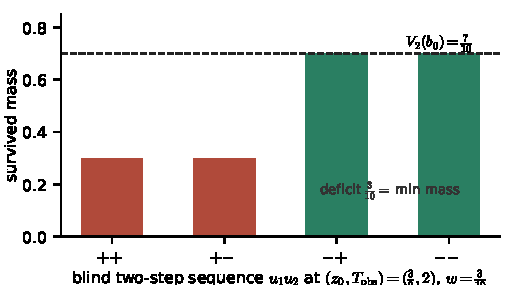
\includegraphics[width=\linewidth]{figs_bs2/fig_masses.pdf}
\caption{The asymmetric audit: survived mass by blind two-step sequence
at \((\tfrac{3}{2}, 2)\) with \(w = \tfrac{3}{10}\). The best sequences
save the heavy branch only; the deficit \(\tfrac{3}{10}\) is the minimal
mass, attained.}
\label{fig:masses}
\end{figure}

\subsection{Certificates as deficit bounds}\label{deficit}

The obstruction certificates bound the deficit from below.

\begin{proposition}[deficit lower bounds]\label{prop:deficit}
The following hold on the audited instances. (i) \emph{Chance-constrained
common-action bound:} if no single action keeps all compatible states
safe, the deficit is at least the minimal compatible mass. (ii)
\emph{Degenerate minimal-mass bound:} in the deterministic limit the
deficit is at least the minimal mass of the belief, attained whenever
exactly one branch is savable (the two-floor instance attains
\(\delta = \tfrac{1}{2}\); on the delayed grid at
\((z_{0}, T_{\mathrm{obs}}) = (\tfrac{3}{2}, 2)\) every blind sequence
loses a branch, so the deficit is at least the minimal mass
\(\tfrac{3}{10}\) of the audited asymmetric prior, and
Table \ref{tab:masses} shows the bound attained). (iii) \emph{Monotone
deficit:} the deficit is non-decreasing in the horizon on the audited
class, and on the certified nonviability region of the delayed grid the
deficit is constant.
\end{proposition}

\subsection{Agreement on the delayed-regime class}\label{agreement}

The class declaration is part of the model: the blind-window policy may
be required to hold one action throughout the window (the declared hold
class), or may act sequentially without observation, or may act with
open-loop time-variation.

\begin{theorem}[certificate--value agreement]\label{thm:agree}
On all 48 audited cells \((z_{0}, T_{\mathrm{obs}})\) with
\(z_{0} \in \{1.0, 1.1, \dots, 2.5\}\) and
\(T_{\mathrm{obs}} \in \{1, 2, 3\}\), and horizons \(k \le 4\):
(i) the class-restricted alpha-vector recursion of Proposition
\ref{prop:pl} reproduces the closed form of Corollary \ref{cor:closed};
(ii) the certificate partition of the grid coincides with the value
boundaries; (iii) the attaining witness and the value's jump loci trace
the certificate boundary exactly, the jump being exactly
\(\tfrac{1}{2}\) at \(z_{0} = 1 + \min(k, T_{\mathrm{obs}})\) and the
value constant on either side.
\end{theorem}

\begin{proof}[Derivation of the jump loci]
Fix \(T_{\mathrm{obs}}\) and \(k\). On the closed form: if
\(k \le T_{\mathrm{obs}}\) the value is
\(\tfrac{1}{2}(\mathbb{1}[z_{0} \ge 1 + k] + 1)\), the second indicator
being identically one on the grid; it jumps by exactly \(\tfrac{1}{2}\)
at \(z_{0} = 1 + k\). If \(k > T_{\mathrm{obs}}\) the value is
\(\tfrac{1}{2}(1 + \mathbb{1}[z_{0} \ge 1 + T_{\mathrm{obs}}])\),
jumping by exactly \(\tfrac{1}{2}\) at \(z_{0} = 1 + T_{\mathrm{obs}}\).
Both loci are \(z_{0} = 1 + \min(k, T_{\mathrm{obs}})\); between jumps
both expressions are constant in \(z_{0}\). The witness family changes
exactly at the same loci: the attaining one-step vector is \((1, 1)\) on
\(z_{0} \ge 2\) and \((1, 0)\) below, and at horizon \(k\) the change
sits at \(z_{0} = 1 + \min(k, T_{\mathrm{obs}})\) --- in particular at
\(z_{0} = 3\), not \(2\), for \(k = 2\) with \(T_{\mathrm{obs}} \ge 2\).
\end{proof}

\begin{theorem}[class declaration]\label{thm:class}
The declared hold class and the unrestricted sequential blind class
coincide at the one-step horizon. For horizons \(k \ge 2\) they differ
exactly on the timing cells --- those with
\(2 \le z_{0} < 1 + T_{\mathrm{obs}}\) --- and there open-loop
time-variation within the blind window lifts the value to one: an
alternating hold sequence keeps both branches at or above the floor
whenever \(z_{0} \ge 2\), which no constant hold does. On the
common-action cells \(z_{0} < 2\) the restriction costs nothing --- no
blind sequence saves both branches --- and on the viable cells both
classes attain one. On the audited grid the difference comprises exactly
the 12 timing cells at each of \(k = 2, 3, 4\): 36 cell-horizon
combinations (Figure \ref{fig:classdiff}).
\end{theorem}

\begin{proof}[Derivation of Theorem \ref{thm:class}]
At \(k = 1\) both classes choose one blind action, so they coincide. Let
\(k \ge 2\) and write the two branch positions after a blind sequence
\(u_{1:\ell}\), \(\ell = \min(k, T_{\mathrm{obs}})\), as
\(z_{0} \pm \sum_{t} u_{t}\). If \(z_{0} < 2\), some branch sits below
\(2 - (z_{0} - 1)\) steps from its floor, and since the partial sums of
any \(\pm1\)-sequence move one branch down whenever they move the other
up, one branch reaches its floor: no blind sequence saves both, both
classes give \(\tfrac{1}{2}\), no difference. If
\(z_{0} \ge 1 + T_{\mathrm{obs}}\) the constant hold already survives
the window on both branches and both classes attain one. On the timing
cells \(2 \le z_{0} < 1 + T_{\mathrm{obs}}\): a constant hold drives the
falling branch to \(z_{0} - \ell < 1\) (deficit), while the alternating
sequence has partial sums in \(\{0, \pm 1\}\), so both branches stay at
or above \(z_{0} - 1 \ge 1\) through the window, and revelation at
\(T_{\mathrm{obs}}\) then regenerates both: the unrestricted class
attains one while the declared class does not. This locates the
difference setwise.
\end{proof}

\begin{figure}[t]
\centering
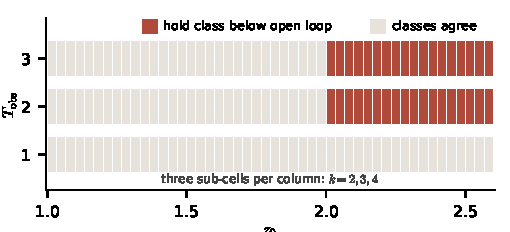
\includegraphics[width=\linewidth]{figs_bs2/fig_classdiff.pdf}
\caption{The class declaration on the audited grid: red cells mark
cell-horizon combinations where the declared hold class and the
unrestricted open-loop class differ --- exactly the timing cells
(\(2 \le z_{0} < 1 + T_{\mathrm{obs}}\)) at horizons \(k = 2, 3, 4\)
(three sub-cells per column); 36 combinations in all. The classes agree
at \(k = 1\), on the common-action cells, and on the viable cells.}
\label{fig:classdiff}
\end{figure}

\subsection{Adaptive observation and hidden parameters}\label{adaptive}

Observation is a design variable. On the declining instance the state
carries a hidden parameter \(\theta \in \{-1, +1\}\) gating the
correctable component of a \(-\tfrac{1}{10}\) drift, and the belief
lives on the product \((z, \theta)\); the obstruction is the emptiness
of the joint floor-servable set over \((x, \theta)\) cells.

\begin{proposition}[probes and learning deadlines]\label{prop:learn}
On the audited grid: with \(\theta\) observed, every cell is viable
(16 of 16). Under one-probe endogenous learning, the probe reveals
\(\theta\) exactly --- the branch separation is \(2\), so one
observation splits the belief with no statistics --- but survival
forces \(z_{0} \ge 21/10\). Under exogenous revelation at horizon
\(T_{\mathrm{learn}}\), viability holds exactly when
\[
z_{0} \;\ge\; \frac{21}{10} \;+\; \frac{T_{\mathrm{learn}}}{10},
\qquad T_{\mathrm{learn}} = 0, 1, 2, 3, 4,
\]
the learning-deadline identity: late resolution acts as the timing
obstruction's observation deadline, and the kernel shrinks exactly
linearly and antitone in it, \(|K| = 5, 4, 3, 2, 1\) on the grid for
\(T_{\mathrm{learn}} = 0, 1, 2, 3, 4\) (Table \ref{tab:deadline} and
Figure \ref{fig:deadline}). A two-patch instance with unknown
regeneration rate \(g \in \{1, 2\}\) shows the same phenomenon on the
audited two-patch belief pair: unknown-regeneration nonviable,
\((x, g)\)-observed viable.
\end{proposition}

\begin{table}[t]
\centering
\footnotesize
\caption{The learning-deadline audit: the exact threshold
\(\tfrac{21}{10} + \tfrac{T_{\mathrm{learn}}}{10}\) and the resulting
kernel on the grid at each deadline.}
\label{tab:deadline}
\begin{tabular}{@{}l c c l@{}}
\toprule
\(T_{\mathrm{learn}}\) & Threshold & \(|K|\) & Kernel \(K\) on the grid\\
\midrule
0 & $21/10$ & 5 & $\{2.1, 2.2, 2.3, 2.4, 2.5\}$\\
1 & $22/10$ & 4 & $\{2.2, 2.3, 2.4, 2.5\}$\\
2 & $23/10$ & 3 & $\{2.3, 2.4, 2.5\}$\\
3 & $24/10$ & 2 & $\{2.4, 2.5\}$\\
4 & $25/10$ & 1 & $\{2.5\}$\\
\bottomrule
\end{tabular}
\end{table}

\begin{figure}[t]
\centering
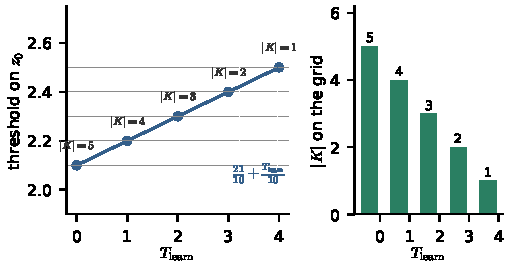
\includegraphics[width=\linewidth]{figs_bs2/fig_deadline.pdf}
\caption{The learning-deadline identity: the viability threshold
increases exactly linearly in \(T_{\mathrm{learn}}\) (left), and the
kernel on the grid shrinks linearly and antitone, \(|K| = 5, 4, 3, 2,
1\) (right).}
\label{fig:deadline}
\end{figure}

\begin{figure}[t]
\centering
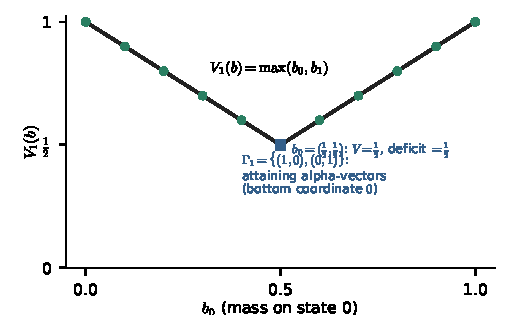
\includegraphics[width=0.88\linewidth]{figs_bs2/fig_twofloor.pdf}
\caption{The two-floor chance instance: the one-step value is
\(\max(b_{0}, b_{1})\), attained by the alpha-vectors of
\(\Gamma_{1} = \{(1,0), (0,1)\}\) with zero bottom coordinate (green
probes); at the symmetric prior the value is \(\tfrac{1}{2}\) and the
deficit equals the minimal mass.}
\label{fig:twofloor}
\end{figure}

\subsection{Verification methods}\label{methods}

Every value, bound, identity, threshold, figure, and tabulated entry in
this paper is regenerated by deterministic scripts in exact integer and
rational arithmetic, standard library only. Two per-system scripts cover
the audited instances --- fifteen check families on the stochastic values
(the two-floor instance, piecewise-linearity, the deterministic limit,
the 48-cell agreement, the partition coincidence, the witness family,
the deficit identity, the unrestricted class, rationality of all 384
campaign alpha-vectors, deficit monotonicity, the oscillation identity,
model completeness, the selector split, dimension consistency, and the
jump loci) and six check families on the adaptive-observation instance
(theta observed, the probe threshold, the learning-deadline identity,
injective revelation, the antitone kernel chain, and the
unknown-regeneration instance). A master script chains the two, then
recomputes independently from the definitions: the closed-form grid
values are reproduced by direct branch-mass enumeration for every cell
with \(k \le T_{\mathrm{obs}}\), the alpha-vector recursion is
re-derived and matched against the closed form on all 192 audited
combinations, the class-difference set is re-enumerated by brute force
(36 combinations), the jump loci are recomputed from the closed form on
the grid, the 384-vector type census (\(156\), \(156\), \(72\)) is
re-derived, every entry of Tables \ref{tab:campaign}, \ref{tab:masses},
and \ref{tab:deadline} is projected against the recomputation, and every
headline number is asserted present in the text. A companion
figure-and-table script recomputes and asserts each plotted or printed
quantity from the same primitives before drawing; the two scripts agree
on every shared quantity.

\subsection{Conclusion}\label{conclusion}

The belief-state safety value carries the obstruction calculus into the
probabilistic setting without loss of exactness. The support identity
ties the value-one level to the viable-set recursion; rational
alpha-vectors keep every audited value exact, and the complete value
table shows the two-valued structure the certificates predict; the
certificates survive as deficit lower bounds, attained on natural
instances on both the symmetric and the asymmetric prior; the audited
delayed-regime class agrees with its closed form cell by cell, with the
class declaration responsible for exactly the 36 timing combinations;
and the adaptive-observation audit prices late resolution exactly --- a
linear learning deadline on the viable set, \(|K| = 5, 4, 3, 2, 1\). The
observation layer, not the forecast layer, sets the value; the design
rules are the same ones the deterministic audits impose, now with a
price attached and every number in the tables open to script-level
re-inspection.

\subsection*{References}

Abaee, A. An obstruction calculus for viability under incomplete
observation (submitted).

Abaee, A., 2026a. Robust viability of the 2J3KL limit reference point
under a surplus-production map: policy scoring, expansion, and when
catch cannot help. Zenodo.
\url{https://doi.org/10.5281/zenodo.22552060}

\subsection*{Declarations}

\subsection*{Funding}
None.

\subsection*{Competing interests}
None.

\subsection*{Data availability}
No external data were used.

\subsection*{Code availability}
The verification script \url{paper2_belief_state_v2_verification.py} and
the figure-and-table generation script
\url{paper2_belief_state_figures.py} are publicly available at
\url{https://github.com/MIKEAA2020/general-sustainability} (folder
\texttt{arena agent 1/paper rewrites/latex}); they reproduce all values,
bounds, thresholds, figures, and tabulated entries verbatim.

\subsection*{AI declaration}
GLM (Z.ai), Qwen (Alibaba Cloud) and DeepSeek AI assisted with drafting
and iterative review. The author reviewed and edited outputs and takes
responsibility for the final work.

\end{document}
